\chapter{Introduzione}
\pagestyle{plain}
Questa tesi si propone di esplorare l'uso della Realtà Mista (MR) in un contesto culinario, con particolare attenzione all'uso di visori come gli HoloLens 2.\\ L'obiettivo principale è quello di sviluppare un'applicazione che possa aiutare a creare ricette con ingredienti inutilizzati evitando anche lo spreco alimentare. Tutto ciò riassunto in un'applicazione semplice e intuitiva che utilizza la MR per sovrapporre informazioni digitali al mondo reale, così da avere pieno controllo di quello che si fa e allo stesso tempo avere le mani libere da qualsiasi dispositivo fisico.\\
L'applicazione è stata sviluppata utilizzando Unity e il Mixed Reality Toolkit (MRTK), che forniscono gli strumenti necessari per creare esperienze MR. Inoltre, utilizzando L'LLM Google Gemini è possibile generare ricette in base agli ingredienti disponibili facendo una semplice foto, rendendo l'applicazione ancora più utile e versatile.
\begin{figure}[]
    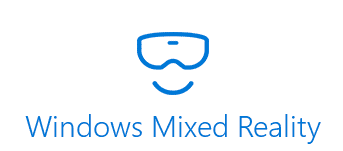
\includegraphics{figures/chapter_1/Windows_Mixed_Reality_logo.png}
    \centering
\end{figure}


